\lab{Numerical Derivatives}{Numerical Derivatives}
\label{lab:NumericalDerivatives}

\objective{Understand and implement finite difference approximations of the derivative in single and multiple dimensions. Evaluate the accuracy of these approximations.  Then use finite difference quotients to find edges in images via the Sobel filter.}

\section*{Derivative Approximations in One Dimension}
The derivative of a function $f$ at a point $x_0$ is

\begin{equation}
\label{eqn:deriv}
f'(x_0) = \lim_{h\rightarrow 0} \frac{f(x_0 + h)-f(x_0)}{h}.
\end{equation}
In this lab, we will investigate one way a computer can calculate $f'(x_0)$. 

\subsection*{Forward Difference Quotient}
Suppose that in Equation \ref{eqn:deriv}, instead of taking a limit, we just pick a small value for $h$. 
Then we would expect $f'(x_0)$ to be close to the quantity
\begin{equation}\label{equ:forward_diff}
 \frac{f(x_0 + h)-f(x_0)}{h}.
\end{equation}
This quotient is called the \emph{first order forward difference approximation} of the derivative. 
Because $f'(x_0)$ is the limit of such quotients, we expect that when $h$ is small, this quotient is close to $f'(x_0)$. 
We can use Taylor's formula to find just how close.

By Taylor's formula,
\[
f(x_0+h) = f(x_0) + f'(x_0)h + R_2(h),
\]
where $R_2(h) = \left( \int_0^1 (1-t) f''(x_0+th) dt \right) h^2$. 
(This is called the \emph{integral form} of the remainder for Taylor's Theorem; see Volume 1 Chapter 6). When we solve this equation for $f'(x_0)$, we get
\begin{equation}\label{equ:forward_diff_with_remainder}
f'(x_0) = \frac{f(x_0+h)-f(x_0)}{h} - \frac{R_2(h)}{h}.
\end{equation}
Thus, the error in using the first order forward difference quotient to approximate $f'(x_0)$ is 
\[
\left | \frac{R_2(h)}{h} \right | \leq |h| \int_0^1 |1 - t||f''(x_0+th)|dt.
\]
If we assume $f''$ is continuous, then for any $\delta$, set $M = \sup_{x \in (x_0-\delta, x_0+\delta)} f''(x)$. Then if $|h| < \delta$, we have
\[
\left | \frac{R_2(h)}{h} \right | \leq |h|\int_0^1 M dt = M|h|  {\in}  O(h).
\]
Therefore, the error in using \eqref{equ:forward_diff} to approximate $f'(x_0)$ grows like $h$.



\subsection*{Centered Difference Quotient}
In fact, we can approximate $f'(x_0)$ to the second order with another difference quotient, called the \emph{centered difference quotient}.  We begin by trying to find the \emph{backward difference quotient}.
Evaluate Taylor's formula at $x_0-h$ to derive
\begin{equation}\label{equ:backwards_diff_with_remainder}
f'(x_0) = \frac{f(x_0)-f(x_0-h)}{h} + \frac{R_2(-h)}{h}.
\end{equation}
The quotient that is the first term on the right hand side of \eqref{equ:backwards_diff_with_remainder} is called the \emph{backward difference quotient.} 
This quotient also approximates $f'(x_0)$ to first order, so it is not the quotient we are looking for.
When we add \eqref{equ:forward_diff_with_remainder} and \eqref{equ:backwards_diff_with_remainder} and solve for $f'(x_0)$ (by dividing by 2), we get
\begin{equation}\label{equ:centered_diff}
f'(x_0) = \frac{\frac{1}{2}f(x_0+h) - \frac{1}{2}f(x_0-h)}{h} + \frac{R_2(-h) - R_2(h)}{2h}
\end{equation}
The \emph{centered difference quotient} is the first term of the right hand side of \eqref{equ:centered_diff}. 
Let us investigate the remainder term to see how accurate this approximation is. 
Recall from the proof of Taylor's theorem that $R_k = \frac{f^{(k)}(x_0)}{k!}h^k + R_{k+1}$. Therefore,
\begin{align*}
\frac{R_2(-h) - R_2(h)}{2h} &= \frac{1}{2h}\left(\frac{f''(x_0)}{2}h^2 + R_{3}(-h) - \frac{f''(x_0)}{2}h^2 - R_{3}(h) \right)\\
&= \frac{1}{2h} ( R_3(-h)-R_3(h))\\
&= \frac{1}{2h}\left(  \left( \int_0^1 \frac{(1-t)^2}{2} f'''(x_0+th) dt \right) h^3  -  \left(\int_0^1 \frac{(1-t)^2}{2} f'''(x_0-th) dt \right) h^3  \right)\\
&= \left(  \int_0^1 \frac{(1-t)^2}{4}( f'''(x_0+th)-f'''(x_0-th)) \right)h^2\\
&{\in}   O(h^2)
\end{align*}
once we restrict $h$ to some $\delta$-neighborhood of 0. 
So the error in using the centered difference quotient to approximate $f'(x_0)$ grows like $h^2$, which is smaller than $h$ when $|h|<1$.

\subsection*{Accuracy of Approximations}

Let us discuss what step size $h$ we should plug into the difference quotients to get the best approximation to $f'(x_0)$.
Since $f'$ is defined as a limit as $h \rightarrow 0$, you may think that it is best to choose $h$ as small as possible, but this is not the case.
In fact, dividing by very small numbers causes errors in floating point arithmetic.
This means that as we decrease $|h|$, the error between $f'(x_0)$ and the difference quotient will first decrease, but then increase when $|h|$ gets too small because of floating point arithmetic. 

Here is an example with the function $f(x) = e^x$. A quick way to write $f$ as a function in Python is with the \li{lambda} keyword. 
\begin{lstlisting}
>>> import numpy as np
>>> from matplotlib import pyplot as plt
>>> f = lambda x: np.exp(x)
\end{lstlisting}
In general, the line \li{f = lambda <params> : <expression>} is equivalent to defining a function \li{f} that accepts the parameters \li{params} and returns \li{expression}.

Next we fix a step size \li{h} and define an approximation to the derivative of \li{f} using the \emph{centered difference quotient}.
\begin{lstlisting}
>>> h = 1e-1
>>> Df_app = lambda x: .5*(f(x+h)-f(x-h))/h
\end{lstlisting}
Finally, we check the accuracy of this approximation at $x_0=1$ by computing the difference between \li{Df_app(1)} and the actual derivative evaluated at 1.
\begin{lstlisting}
# Since f(x) = e^x, the derivative of f(x) is f(x)
>>> np.abs( f(1)-Df_app(1) )
0.0045327354883726301
\end{lstlisting}
We note that our functions \li{f} and \li{Df_app} behave as expected when they are passed a NumPy array.
\begin{lstlisting}
>>> h = np.array([1e-1, 1e-3, 1e-5, 1e-7, 1e-9, 1e-11])
>>> np.abs( f(1)-Df_app(1) )
array([  4.53273549e-03,   4.53046679e-07,   5.85869131e-11,
         5.85873572e-11,   6.60275079e-09,   1.04294937e-05])
\end{lstlisting}
These results are summarized in Table \ref{table:approx_errors}.

\begin{table}
\begin{center}
\begin{tabular}{|c|c|c|c|c|c|c|}
\hline
$h$ 		& 1e-1 & 1e-3 & 1e-5 & 1e-7	 & 1e-9 & 1e-11 \\ \hline
Error  	& 5e-3 & 5e-7 & 6e-11 & 6e-11 & 7e-9 & 1e-5\\ \hline
\end{tabular}
\caption{This table shows that it is best not to choose $h$ too small when you approximate derivatives with difference quotients. 
Here, ``Error'' equals the absolute value of $f'(1)-f_{app}(1)$ where $f(x) = e^x$ and $f_{app}$ is the centered difference approximation to $f'$.}
\label{table:approx_errors}
\end{center}
\end{table}

Thus, the optimal value of $h$ is one that is small, but not too small. A good choice is \li{h = 1e-5}.

\begin{problem}
Write a function that accepts as input a callable function object \li{f}, an array of points \li{pts}, and
a keyword argument \li{h} that defaults to \li{1e-5}. 
Return an array of the \emph{centered difference quotients} of \li{f} at each point in \li{pts} with the specified value of \li{h}.
\end{problem}
\begin{problem}
Write a function that accepts as input a callable function object \li{f}, an array of points \li{pts}, and
a keyword argument \li{h} that defaults to \li{1e-5}.  Return an array of the errors for the \emph{centered difference quotients} at each point in \li{pts} with the specified value of \li{h}.
\end{problem}

You may wonder if the forward or backward difference quotients are ever used, since the centered difference quotient is a more accurate approximation of the derivative.
In fact, there are some functions that in practice do not behave well under centered difference quotients.
In these cases, one must use the forward or backward difference quotient.


Finally, we remark that forward, backward, and centered difference quotients can be used to approximate higher-order derivatives of $f$.
However, taking derivatives is an \emph{unstable} operation. 
This means that taking a derivative can amplify the arithmetic error in your computation.
For this reason, difference quotients are not generally used  to approximate derivatives higher than second order.





\begin{comment}
The derivative of a function at a point is formally defined as

\begin{equation}
\label{eqn:deriv}
f'(x) = \lim_{h\rightarrow 0} \frac{f(x + h)-f(x)}{h}.
\end{equation}

In most real world applications we will be solving problems using computers. How does a computer calculate a limit? In short it can't. Computers can only approximate functions at specific points, and the notion of a limit graces infinity in a way that a computer never can.

So how can we use a computer to find the derivative of a function, particularly when we can't differentiate the function by hand? We use methods known as finite difference methods. For example suppose that in equation \ref{eqn:deriv}, instead of taking a limit we just pick a particularly small value for h. Then we have

\begin{equation*}
f'(x) \approx \frac{f(x + h)-f(x)}{h}
\end{equation*}

This is known as the first order forward difference approximation of the derivative.

How do we know the quality of this approximation? We can use Taylor's formula to find

\begin{equation*}
f(x_0 + h) = f(x_0) + hf'(x_0) + h^2/2 f''(\xi),\hspace{5mm} \xi \in (x_0,x_0 + h)
\end{equation*}

Which can be also expressed as

\begin{equation*}
f'(x_0) = \frac{f(x_0 + h) - f(x)}{h} + \frac{h}{2}f''(\xi) = \frac{f(x_0 + h) - f(x)}{h} + O(h)
\end{equation*}

Here we use the big-O notation to denote that the errors are bounded by some constant multiplied by $h$.

We can use Taylor expansions to find approximations that have different big-O error bounds, up to any polynomial of arbitrary degree. Tables \ref{Table:CDiff} and \ref{Table:FDiff} offer the coefficients for centered and forward difference schemes.

\begin{table}
\begin{center}
\begin{tabular}{|c|c|c|c|c|c|c|c|c|}
\hline
Derivative & Accuracy & -3 & -2 & -1 & 0 & 1 & 2 & 3 \\ \hline
 & 2 & & & -1/2 & 0 & 1/2 & & \\ \cline{2-9}
 1 & 4 & & 1/12 & -2/3 &  0 & 2/3 & -1/12 & \\ \cline{2-9}
  & 6 & -1/60 & 3/20 & -3/4 & 0 & 3/4 & -3/20 & 1/60 \\ \hline
  & 2 & & & 1 & -2 & 1 & & \\ \cline{2-9}
 2 & 4 & & -1/12 & 4/3 &  -5/2 & 4/3 & -1/12 & \\ \cline{2-9}
  & 6 & 1/90 & -3/20 & 3/2 & -49/18 & 3/2 & -3/20 & 1/90 \\ \hline
\end{tabular}
\caption{Centered Difference Coefficients}
\label{Table:CDiff}
\end{center}
\end{table}

\begin{table}
\begin{center}
\begin{tabular}{|c|c|c|c|c|c|c|}
\hline
Derivative & Accuracy & 0 & 1 & 2 & 3 & 4 \\ \hline
 & 1 & -1 & 1 &  & &  \\ \cline{2-7}
 1 & 2 & -3/2 & 2 & -1/2 & &  \\ \cline{2-7}
  & 3 & -11/6 & 3 & -3/2 & 1/3 &  \\ \hline
  & 1 & 1 & -2 & 1 &  & \\ \cline{2-7}
 2 & 2 & 2 & -5 & 4 &  -1 &  \\ \cline{2-7}
  & 3 & 35/12 & -26/3 & 19/2 & -14/3 & 11/12 \\ \hline
\end{tabular}
\caption{Forward Difference Coefficients}
\label{Table:FDiff}
\end{center}
\end{table}

These tables can be used by simply summing the function evaluations (the number at the top represents how many times $h$ is added to $x$), and then dividing by $h^n$, where $n$ is the degree of the derivative.

So, for example, the centered difference estimate of the second derivative that is $O(h^4)$ is
\begin{equation*}
f''(x) \approx \frac{-1/12(f(x-2h) + f(x+2h)) + 4/3(f(x-h) + f(x+h)) -5/2f(x)}{h^2}
\end{equation*}

Or, the forward difference estimate for the first derivative that is $O(h^2)$ is

\begin{equation*}
f'(x) \approx \frac{-3/2f(x) + 2f(x+h) - 1/2 f(x+2h)}{h}
\end{equation*}

It should be noted that we can convert a forward difference estimate to a backwards difference estimate by using $-h$. So the backwards difference estimate for the first derivative that is $O(h^2)$ is

\begin{equation*}
f'(x) \approx \frac{3/2f(x) - 2f(x-h) + 1/2 f(x-2h)}{h}
\end{equation*}

There are two important observations that you should make about these tables. First, in order to get higher order approximations we need to evaluate the function at more points. This should not be surprising. Second, you should notice that centered difference formulas require less function evaluations to get higher order approximations. However, in certain applications it is not possible to use centered difference formulas, so the backwards and forwards formulas are still very applicable.

One important aspect of this method is selecting an appropriate $h$. The natural temptation is to pick a very very small value. However, this is not always advisable. Note the values in table \ref{Table:FloatingError}, which approximates the derivative of $e(x)$ at $x = 1$:

\begin{table}[h!]
\begin{center}
\begin{tabular}{|cc|}
\hline
h & Error  = $|f'(1)-f'_{app}(1)|$ \\ \hline
1e-1 & 4.5e-3 \\
1e-3 & 4.5305e-7 \\
1e-7 & 5.8587e-11 \\
1e-10 & 6.7274e-7 \\ \hline
\end{tabular}
\caption{Error in numerical derivative, using double precision floating point arithmetic}
\label{Table:FloatingError}
\end{center}
\end{table}

As you can see, the error actually increases as $h$ becomes very small. Why is this? Division by small numbers causes errors in floating point arithmetic. So, be aware that usually the optimal $h$ is of moderately small size. However, in the framework of double floating point arithmetic, this is usually less of a concern.

As a matter of reference, calculating numerical derivatives is an unstable operation. An unstable operation, informally, is one where errors are magnified by the operation. This usually is not an issue, but it's important to know that taking derivatives can amplify errors.

\begin{problem}
Write a function \li{numDer1} that accepts as inputs: a callable function object \li{f} and
a keyword argument \li{h} giving the step size (default \li{h = 1e-5}). Have the function return an array of the approximate 1st order derivative with accuracy 1 of \li{f} at each of the points in \li{pts}, using the centered  coefficients.
\end{problem}

\begin{problem}
Write a function \li{numDer2} that accepts as inputs: a callable function object \li{f} and
a keyword argument \li{h} giving the step size (default \li{h = 1e-5}). Have the function return an array of the approximate 2nd order derivative with accuracy 1 of \li{f} at each of the points in \li{pts}, using the centered  coefficients.
\end{problem}


\begin{problem}
Write a function \li{numDer} that accepts as inputs: a callable function object \li{f}, an
array of numbers \li{pts}, a keyword argument \li{mode} (taking one of the values 
\li{'centered'}, \li{'forward'}, or \li{'backward'}), a keyword argument \li{d} (taking one of 
the values \li{1} or \li{2}), a keyword argument \li{o} (taking an integer value in 
\li{[2, 4, 6]} if \li{mode = 'centered'}, and otherwise taking a value in \li{[1, 2, 3]}), and
a keyword argument \li{h} giving the step size. The default settings of the keyword
arguments should be \li{mode = 'centered', d = 1, o = 2, h = 1e-5}.
 
Have the function return an array of the approximate derivative of order \li{d} with accuracy
 \li{o} of \li{f} at each of the points in \li{pts}, using the coefficients indicated by \li{mode}.
\end{problem}


We note that higher order approximations of the derivative can be derived using the Taylor series and Lagrange polynomials, but generally higher-order approximations are not practically useful as they can often be ill-conditioned.

For any numerical approximation method, it is important to be able to empirically calculate
the order of convergence. We will do so for our numerical derivative approximation. 
For an $m$-th order approximation of the first derivative, we have that the error is in
$O(h^m)$, so that
$$
err(h) \approx Ch^m
$$
for some constant $C$.
Hence, taking the log of both sides, we obtain
$$
\log err(h) \approx \log C + m\log h,
$$
which means that if we plot the log of the errors against the log of the $h$ values, we 
ought to see a linear relationship whose slope gives the rate of convergence. 

We do this in python as follows (The \li{numDer} function in this code can use any of the coefficients from \ref{Table:CDiff} and \ref{Table:FDiff}):
\begin{lstlisting}
# assume that the function numDer has already been written
import numpy as np
from matplotlib import pyplot as plt

# approximate the derivative of cosine at x = 3
# create a callable function object
def myCosine(x):
    return np.cos(x)
f = myCosine

# calculate the actual derivative
actual = -np.sin(3.0)

# initialize array of h values at which to calculate the error
hvals = np.linspace(1e-5, 1e-1)
err1 = np.zeros(hvals.shape)
err2 = np.zeros(hvals.shape)

# calculate the errors for order 1 and order 2 approximations for the forward coeffiects
for i in xrange(len(hvals)):
    err1[i] = np.abs(actual - numDer(f, np.array([3.0]), mode = 'forward', h = hvals[i], o=1))
    err2[i] = np.abs(actual - numDer(f, np.array([3.0]), mode = 'forward', h = hvals[i], o=2))

# plot the log of the h values against the log of the errors
plt.subplot(121)
plt.loglog(hvals, err1)
plt.ylim((1e-11, 1e-1))
plt.subplot(122)
plt.loglog(hvals, err2)
plt.ylim((1e-11, 1e-1))
plt.show()
\end{lstlisting}

The generated plot is shown in Figure \ref{fig:convergence}. Note that the slope
of the line in the left plot is about 1, and the slope of the line in the right
plot is about 2. Further, the log of the errors for the order 2 approximations
are much lower than the log of the errors of the order 1 approximations.

\begin{figure}[t]
    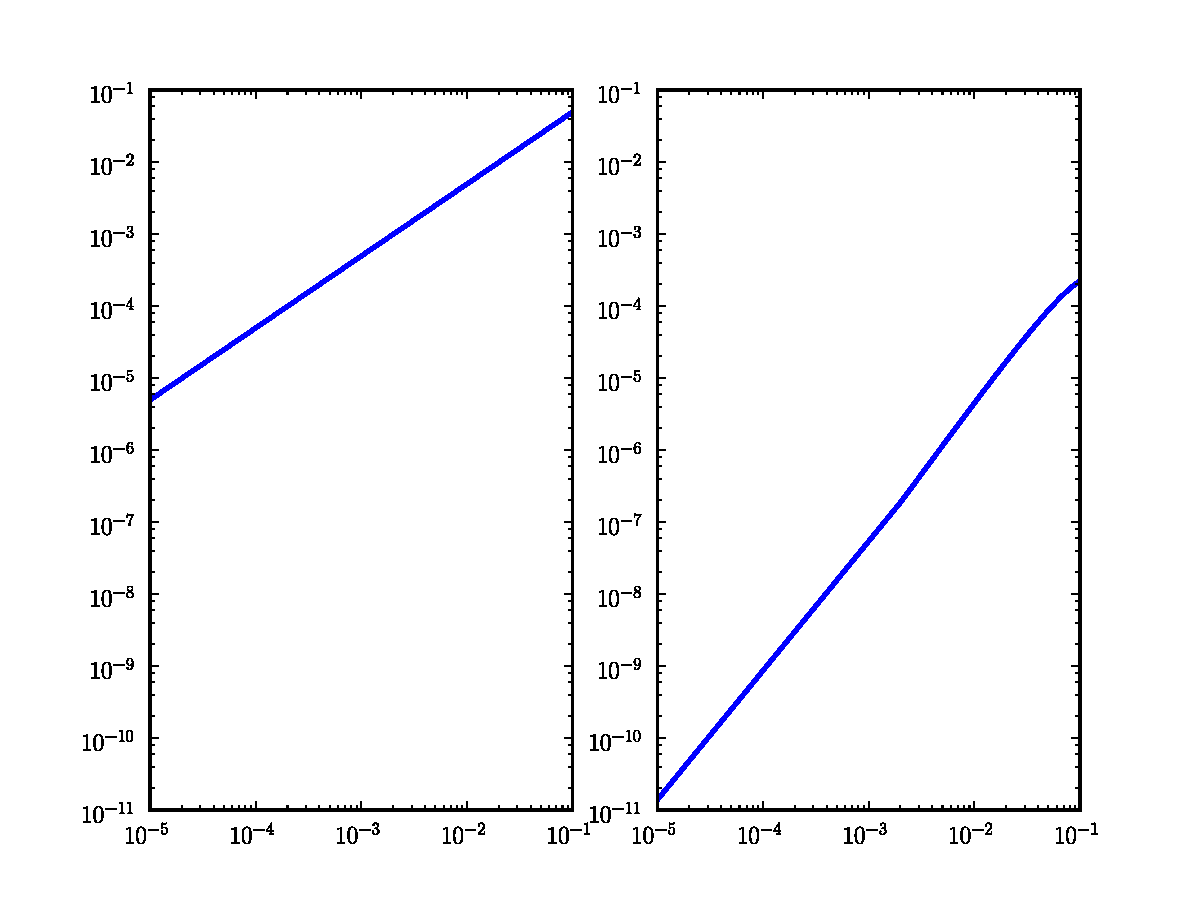
\includegraphics[width=0.8\textwidth]{convergence.pdf}
    \caption{Convergence plots for our numerical derivative approximations.
    The left plot shows the convergence for order 1 approximations. 
    The right plot shows the convergence for order 2 approximations.}
    \label{fig:convergence}
\end{figure}


\begin{problem}
Explore the convergence properties for different orders of approximation,
and for the second derivative as well. You may need to adjust your $h$
values, as they may be too small for some of the calculations.
\end{problem}

\end{comment}
\section*{Derivative Approximations in Multiple Dimensions}
Finite difference methods can also be used to calculate derivatives in higher dimensions.
Recall that the Jacobian of a function $f:\mathbb{R}^n \rightarrow \mathbb{R}^m$ at a point $x_0 \in \mathbb{R}^n$ is the $m \times n$ matrix $J = (J_{ij})$ defined component-wise by
\begin{equation*}
J_{ij} = \frac{\partial f_i}{\partial x_j}(x_0).
\end{equation*}
For example, the Jacobian for a function $f:\mathbb{R}^3 \rightarrow \mathbb{R}^2$ is defined by

\[
J = \begin{pmatrix}
\frac{\partial f}{\partial x_1}&\frac{\partial f}{\partial x_2}&\frac{\partial f}{\partial x_3}
\end{pmatrix}
= \begin{pmatrix}
\frac{\partial f_1}{\partial x_1}&\frac{\partial f_1}{\partial x_2}&\frac{\partial f_1}{\partial x_3}\\
\frac{\partial f_2}{\partial x_1}&\frac{\partial f_2}{\partial x_2}&\frac{\partial f_2}{\partial x_3}
\end{pmatrix}.
\]

The Jacobian is useful in many applications.  For example, the Jacobian can be used to find zeros of functions in multiple variables.



The forward difference quotient for approximating a partial derivative is
\begin{equation*}
\frac{\partial f}{\partial x_j} (x_0) \approx \frac{f(x_0+h e_j)-f(x_0)}{h},
\end{equation*}
where $e_j$ the $j^{th}$ standard basis vector. 
Similarly, the centered difference approximation is
\begin{equation*}
\frac{\partial f}{\partial x_j} (x_0) \approx \frac{\frac{1}{2}f(x_0+h e_j)-\frac{1}{2}f(x_0-h e_j)}{h}.
\end{equation*}

\begin{problem}
\leavevmode
Write a function that accepts 
\begin{enumerate}
\item a function handle \li{f},
\item an integer \li{n} that is the dimension of the domain of \li{f},
\item an integer \li{m} that is the dimension of the range of \li{f},
\item an \li{n}-dimensional NumPy array \li{pt} representing a point in $\mathbb{R}^n$, and
\item an keyword argument \li{h} that defaults to \li{1e-5}.
\end{enumerate}
Return the approximate Jacobian matrix of \li{f} at \li{pt} using the centered difference quotient.
\end{problem}
\begin{problem}
\item Let $f: \mathbb{R}^2 \to \mathbb{R}^2$ be defined by
\begin{equation*}
f(x, y) =
\begin{pmatrix}
e^{x} \sin(y) + y^3 \\
3y - \cos(x)
\end{pmatrix}
\end{equation*}
Find the error between your Jacobian function and the analytically computed derivative on the square $[-1,1] \times [-1,1]$ using ten thousand grid points (100 per side).
You may apply your Jacobian function to the points one at a time using a double \li{for} loop.  Once you get the error matrix for a given point, calculate the Frobenius norm of this matrix (\li{la.norm} defaults to the Frobenius norm).  This norm will be your total error for that point.
What is the maximum error of your Jacobian function over all points in the square?

Hint: The following code defines the function
$f(x,y) = 
\begin{pmatrix}
x^2\\
x+y
\end{pmatrix}$.
\begin{lstlisting}
# f accepts a length-2 NumPy array
>>> f = lambda x: np.array([x[0]**2, x[0]+x[1]])
\end{lstlisting}
\end{problem}

\begin{comment}
Given a function from $\mathbb{R}^n \to \mathbb{R}$, sometimes the mixed partial derivatives are useful. In particular, the mixed partials will be useful when we study optimization in Volume 2. This information is contained in the Hessian matrix, which is defined as

\begin{equation*}
H_{ij} = \frac{\partial^2 f}{\partial x_i \partial x_j}
\end{equation*}

We can use the following formula to approximate mixed partial derivatives
\small
\begin{equation*}
\frac{\partial^2 f}{\partial x_i \partial x_j} = \frac{f(x + (e_i + e_j)h) - f(x + (e_i-e_j)h) -f(x + (e_j-e_i)h) + f(x - (e_i + e_j)h)}{4h^2}
\end{equation*}
\normalsize

\begin{problem}
Write a Python function that numerically calculates the Hessian of a given function. 
The function should be named \li{Hessian}, and should accept as inputs a function handle, 
an integer giving the dimension of the domain of the function, a NumPy 
array giving the point at which to approximate the Hessian, and an optional argument giving the 
step size.
Return the approximated Hessian matrix at the given point.

Test it on the following function
\begin{equation*}
f(x,y) = (1-x)^2 + 100(y-x^2)^2
\end{equation*}
This function is known as the Rosenbrock Banana function, or Rosenbrock's Valley. It is a common test function for optimization algorithms because it is non-convex and the global minimum is hard to find from certain starting points. A graph is shown in figure \ref{Fig:Rosenbrock}. Compare the output of your function with the analytic solution on the region $[-2,2] \times [0,2]$, using ten thousand points. What is the maximum error of your function?
\end{problem}
\begin{figure}
\begin{center}
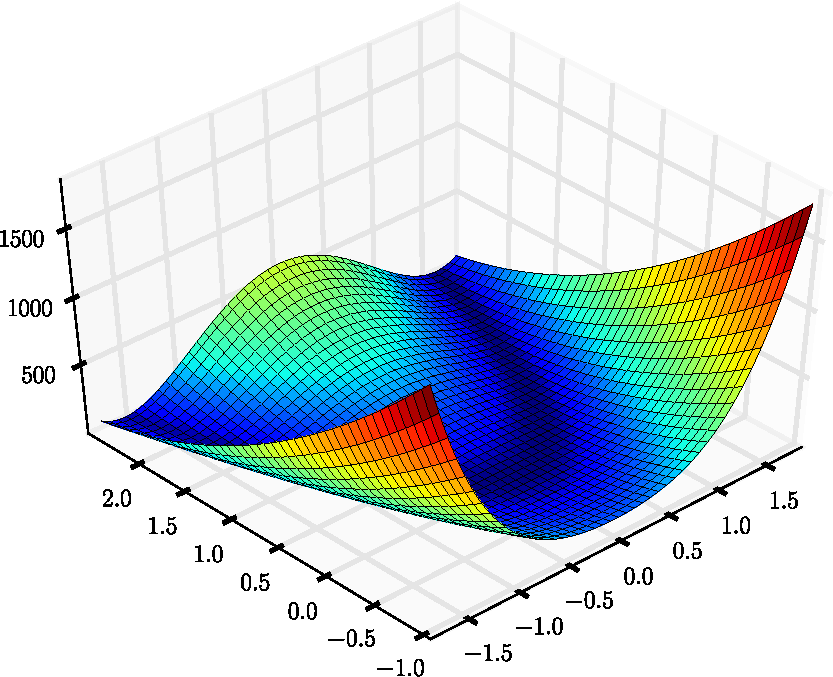
\includegraphics[width = \textwidth]{Rosenbrock}
\caption{The Rosenbrock Banana Function, a common test function in optimization algorithms}
\label{Fig:Rosenbrock}
\end{center}
\end{figure}
\end{comment}

\section*{Application to Image Filters}
Recall that a computer stores an image as a 2-D array of pixel values (i.e., a matrix of intensities).
An image filter is a function that transforms an image by operating on it locally.
That is, to compute the $ij^{th}$ pixel value in the new image, an image filter uses only the pixels in a small neighborhood around the $ij^{th}$ pixel in the original image.

In this lab, we will use a filter derived from the gradient of an image to find edges in an image.

\subsection*{Convolutions}
One example of an image filter is to \emph{convolve} an image with a filter matrix.
A filter matrix is a matrix whose height and width are relatively small odd numbers.
If the filter matrix is
\[
F = \begin{pmatrix}
f_{-1,-1}&f_{-1,0}&f_{-1,1}\\
f_{0,-1}&f_{0,0}&f_{0,1}\\
f_{1,-1}&f_{1,0}&f_{1,1}
\end{pmatrix},
\]
then the convolution of an image $A$ with $F$ is $A \ast F = (C_{ij})$ where
\begin{equation}\label{equ:convolve}
C_{ij} = \sum_{k=-1}^1 \sum_{\ell=-1}^1 f_{k\ell}A_{i+k,j+\ell}.
\end{equation}
Say $A$ is an $m \times n$ matrix. Here, we take $A_{ij}=0$ when $i \not \in \{1, \ldots m\}$ or $j \not \in \{1, \ldots, n\}$.
The value of $C_{ij}$ is a linear combination of the nearby pixel values, with coefficients given by $F$ (see Figure \ref{fig:convolution}).
In fact, $C_{ij}$ equals the Frobenius inner product of $F$ with the $3 \times 3$ submatrix of $A$ centered at $ij$.

\begin{figure}
\centering
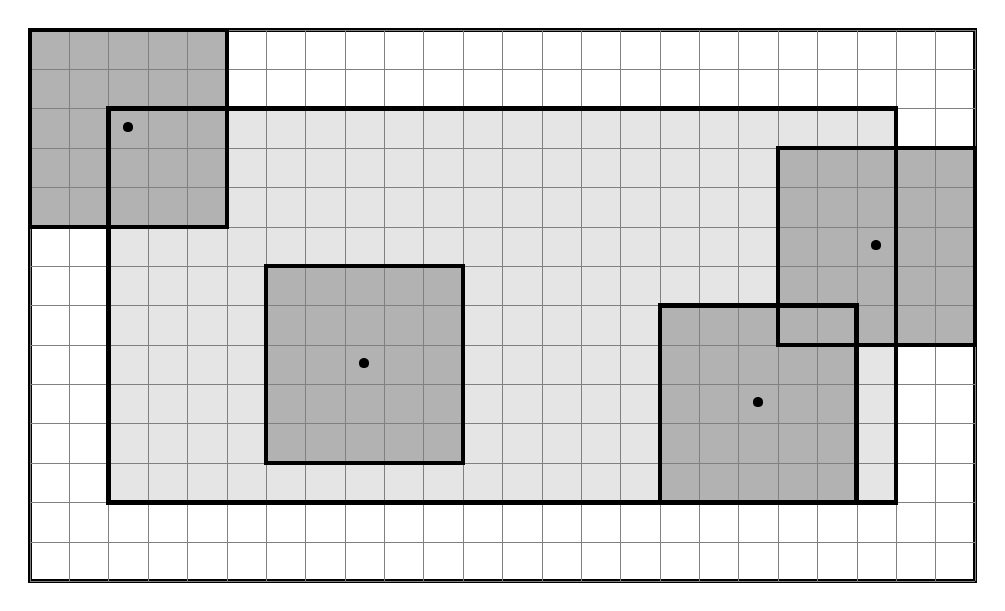
\begin{tikzpicture}
\node[draw, minimum width=12cm, minimum height=
	7cm, ultra thick](outer_rec)[]{};
\node[draw, minimum width=10cm, minimum height=
	5cm, ultra thick, fill=black!10!](inner_rec)[]{};
\node[draw, minimum width=2.5cm, minimum height=2.5cm, 
	ultra thick, fill=black!30!](square1)at(-4.75,2.25){\textbullet};
\node[draw, minimum width=2.5cm, minimum height=2.5cm, 
	ultra thick,fill=black!30!](square2)at(-1.75,-.75){\textbullet};
\node[draw, minimum width=2.5cm, minimum height=2.5cm, 
	ultra thick, fill=black!30!](square3)at(4.75,.75){\textbullet};
\node[draw, minimum width=2.5cm, minimum height=2.5cm, 
	ultra thick, fill=black!30!](square4)at(3.25,-1.25){\textbullet};
\draw[step=.5, ultra thin, color=black!50!](-6,-3.5)grid(6,3.5);

%redraw borders
\node[draw, minimum width=10cm, minimum height=
	5cm, ultra thick, ][]{};
\node[draw, minimum width=2.5cm, minimum height=2.5cm, 
	ultra thick]at(-4.75,2.25){};
\node[draw, minimum width=2.5cm, minimum height=2.5cm, 
	ultra thick]at(-1.75,-.75){};
\node[draw, minimum width=2.5cm, minimum height=2.5cm, 
	ultra thick]at(4.75,.75){};
\node[draw, minimum width=2.5cm, minimum height=2.5cm, 
	ultra thick]at(3.25,-1.25){};
\end{tikzpicture}
\caption{This diagram illustrates how to convolve an image with a filter.
The light grey rectangle represents the original image $A$, and the dark grey squares are the filter $F$.
The larger rectangle is the image padded with zeros; i.e., all pixel values in the outer white band are 0.
To compute the entry of the convolution matrix $C$ located at a black dot, take the inner product of $F$ with the submatrix of the padded image centered at the dot.}
\label{fig:convolution}
\end{figure}

\subsubsection*{Implementation in NumPy}
Let us write a function that convolves an image with a filter. 
You can test this function on the image \li{cameraman.jpg}, which appears in Figure \ref{fig:cameraman}.
The following code loads this image and plots it with matplotlib.
\begin{lstlisting}
>>> image = plt.imread('cameraman.jpg')
>>> plt.imshow(image, cmap = 'gray')
>>> plt.show()
\end{lstlisting}

Here is the function definition and some setup.
\begin{lstlisting}
1. def Filter(image, F):
2.     m, n = image.shape
3.     h, k = F.shape
\end{lstlisting}
To convolve \li{image} with the filter \li{F}, we must first \emph{pad} the array \li{image} with zeros around the edges.
This is because in \eqref{equ:convolve}, entries $A_{ij}$ are set to zero when $i$ or $j$ is out of bounds.
We do this by creating a larger array of zeros, and then making the interior part of the array equal to the original image (see Figure \ref{fig:convolution}).

For example, if the filter is a $3 \times 3$ matrix, then the following code will pad the matrix with the appropriate number of zeros.
\begin{lstlisting}
 # Create a larger matrix of zeros
image_pad = np.zeros((m+2, n+2))
# Make the interior of image_pad equal to the original image
image_pad[1:1+m, 1:1+n] = image
\end{lstlisting}
We want to do this in general in our function.  Note that the number of zeros we need to pad our array depends on the size of the filter \li{F}.
\begin{lstlisting}
5.    image_pad = # Create an array of zeros of the appropriate size
6.   # Make the interior of image_pad equal to image
\end{lstlisting}

Finally, we iterate through the image to compute each entry of the convolution matrix.
\begin{lstlisting}
7.    C = np.zeros(image)
8.    for i in range(m):
9.        for j in range(n):
10.            C[i,j] = # Compute C[i, j]
\end{lstlisting}

\subsubsection*{Gaussian Blur}
A \emph{Gaussian blur} is an image filter that operates on an image by convolving with the matrix
\[
G = \frac{1}{159}\begin{pmatrix}
2&4&5&4&2\\
4&9&12&9&4\\
5&12&15&12&5\\
4&9&12&9&4\\
2&4&5&4&2
\end{pmatrix}.
\]

Blurring an image can remove ``noise'', or random variation that is the visual analog of static in a radio signal (and equally undesirable).

\begin{problem}\label{prob:filter}
\leavevmode
Finish writing the function \li{Filter} by filling in lines 5, 6, and 10.  Hint: Note in \ref{equ:convolve}, $C_{ij}$ was calculated by summing from -1 to 1.  This is only the case if the filter \li{F} is $3 \times 3$. A slight modification is needed in the general case.  Test your function on the image \li{cameraman.jpg} using the Gaussian Blur. The result is in Figure \ref{fig:cameraman_blur}.
\end{problem}


% TODO: make pictures that aren't pdfs
\begin{figure}
\centering
\begin{subfigure}[b]{.49\textwidth}
\centering
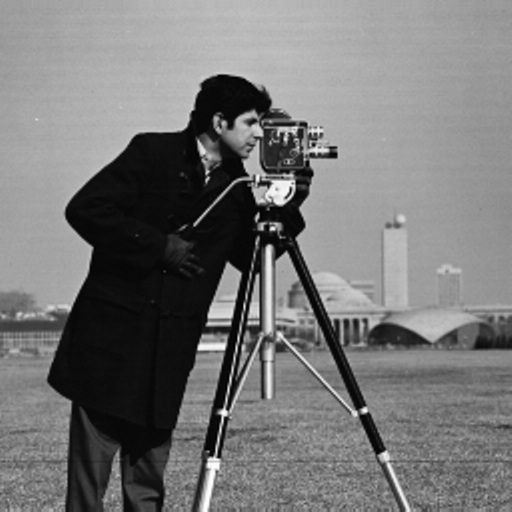
\includegraphics[width=\textwidth]{cameraman.jpg}
\caption{Unfiltered image.}
\label{fig:cameraman}
\end{subfigure}
\begin{subfigure}[b]{.49\textwidth}
\centering
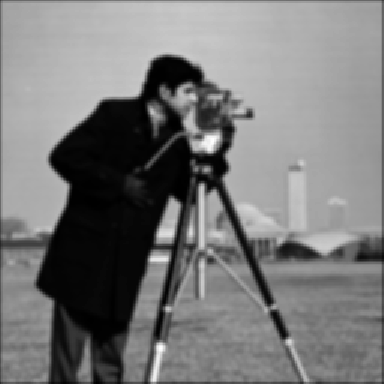
\includegraphics[width=\textwidth]{cameramanBlur.pdf}
\caption{Image after Gaussian blur is applied.}
\label{fig:cameraman_blur}
\end{subfigure}
\begin{subfigure}[b]{.49\textwidth}
\centering

\includegraphics[width=\textwidth]{edges.pdf}
\caption{Image after the Sobel filter is applied.}
\label{fig:cameraman_edges}
\end{subfigure}
\caption{Here is an example of a Gaussian blur and the Sobel filter applied to an image. 
This photo, known as ``cameraman,'' is a standard test image in image processing. 
A database of such images can be downloaded from \url{http://www.imageprocessingplace.com/root_files_V3/image_databases.htm}.}
\label{fig:cameraman1}
\end{figure}



\subsection*{Edge Detection}

Automatically detecting edges in an image can be used to segment or sharpen the image. 
We will find edges with the Sobel filter, which computes the gradient of the image at each pixel. 
The magnitude of the gradient tells us the rate of change of the pixel values, and so large magnitudes should
correspond to edges within the image. 
The Sobel filter is not a convolution, although it does use convolutions.

We can think of an image as a function from a $2 \times 2$ grid of points to $\mathbb{R}$.
The image maps a pixel location to an intensity.
It does not make sense to define the derivative of this function as a limit because the domain is discrete---a step size $h$ cannot take on arbitrarily small values.
Instead, we \emph{define} the derivative to be the centered difference quotient of the previous section.
That is, we define the derivative in the $x$-direction at the $ij^{th}$ pixel to be 
\[
\frac{1}{2}A_{i+1, j} - \frac{1}{2}A_{i-1, j}.
\]

We can use a convolution to create a matrix $A_x$ whose $ij^{th}$ entry is the derivative of $A$ at the $ij^{th}$ entry, in the $x$-direction.
In fact, $A_x = A \ast S$, where
\[
S = \frac{1}{8} \begin{pmatrix}
-1 & 0 & 1\\
-2 & 0 & 2\\
-1 & 0 & 1
\end{pmatrix}.
\]

Note that this convolution takes a weighted average of the $x$-derivatives at $(i, j)$, $(i, j+1)$, and $(i, j-1)$. 
The derivative at $(i, j)$ is weighted by 2.
Using a weighted average instead of just the derivative at $(i, j)$ makes the derivative less affected by noise.

Now we can define the Sobel filter. 
A Sobel filter applied to an image $A$ results in an array $B = (B_{ij})$ of 0's and 1's, where the 1's trace out the edges in the image. 
By definition,
\[
B_{ij} = \left\{
     \begin{array}{ll}
       1 & \text{if}\; \;\|\nabla A(ij)\|_2 > M \\
       0 & \text{otherwise}.
     \end{array}
   \right.
\]
Here, $\nabla A(ij) = ((A \ast S)_{ij}, (A\ast S^T)_{ij})$ is the gradient of $A$ at the $ij^{th}$ pixel.
The constant $M$ should be ``sufficiently large'' enough to pick out those pixels with the largest gradient (i.e., those pixels that are part of an edge).
A good choice for $M$ is 4 times the average value of $\|\nabla A(ij)\|_2$ over the whole image $A$.


When the Sobel filter is applied to \li{cameraman.jpg}, we get the image in Figure \ref{fig:cameraman_edges}. 
Here, the 1's in $B$ were mapped to ``white'' and the 0's were mapped to ``black.''




\begin{problem}
Write a function that accepts an image as input and applies the Sobel filter to the image.  Test your function on \li{cameraman.jpg}.  Hint: If you want to find the average of a matrix \li{A}, use the function \li{A.mean()}.
\end{problem}



